\documentclass[twoside]{book}

% Packages required by doxygen
\usepackage{fixltx2e}
\usepackage{calc}
\usepackage{doxygen}
\usepackage[export]{adjustbox} % also loads graphicx
\usepackage{graphicx}
\usepackage[utf8]{inputenc}
\usepackage{makeidx}
\usepackage{multicol}
\usepackage{multirow}
\PassOptionsToPackage{warn}{textcomp}
\usepackage{textcomp}
\usepackage[nointegrals]{wasysym}
\usepackage[table]{xcolor}

% Font selection
\usepackage[T1]{fontenc}
\usepackage[scaled=.90]{helvet}
\usepackage{courier}
\usepackage{amssymb}
\usepackage{sectsty}
\renewcommand{\familydefault}{\sfdefault}
\allsectionsfont{%
  \fontseries{bc}\selectfont%
  \color{darkgray}%
}
\renewcommand{\DoxyLabelFont}{%
  \fontseries{bc}\selectfont%
  \color{darkgray}%
}
\newcommand{\+}{\discretionary{\mbox{\scriptsize$\hookleftarrow$}}{}{}}

% Page & text layout
\usepackage{geometry}
\geometry{%
  a4paper,%
  top=2.5cm,%
  bottom=2.5cm,%
  left=2.5cm,%
  right=2.5cm%
}
\tolerance=750
\hfuzz=15pt
\hbadness=750
\setlength{\emergencystretch}{15pt}
\setlength{\parindent}{0cm}
\setlength{\parskip}{3ex plus 2ex minus 2ex}
\makeatletter
\renewcommand{\paragraph}{%
  \@startsection{paragraph}{4}{0ex}{-1.0ex}{1.0ex}{%
    \normalfont\normalsize\bfseries\SS@parafont%
  }%
}
\renewcommand{\subparagraph}{%
  \@startsection{subparagraph}{5}{0ex}{-1.0ex}{1.0ex}{%
    \normalfont\normalsize\bfseries\SS@subparafont%
  }%
}
\makeatother

% Headers & footers
\usepackage{fancyhdr}
\pagestyle{fancyplain}
\fancyhead[LE]{\fancyplain{}{\bfseries\thepage}}
\fancyhead[CE]{\fancyplain{}{}}
\fancyhead[RE]{\fancyplain{}{\bfseries\leftmark}}
\fancyhead[LO]{\fancyplain{}{\bfseries\rightmark}}
\fancyhead[CO]{\fancyplain{}{}}
\fancyhead[RO]{\fancyplain{}{\bfseries\thepage}}
\fancyfoot[LE]{\fancyplain{}{}}
\fancyfoot[CE]{\fancyplain{}{}}
\fancyfoot[RE]{\fancyplain{}{\bfseries\scriptsize Generated by Doxygen }}
\fancyfoot[LO]{\fancyplain{}{\bfseries\scriptsize Generated by Doxygen }}
\fancyfoot[CO]{\fancyplain{}{}}
\fancyfoot[RO]{\fancyplain{}{}}
\renewcommand{\footrulewidth}{0.4pt}
\renewcommand{\chaptermark}[1]{%
  \markboth{#1}{}%
}
\renewcommand{\sectionmark}[1]{%
  \markright{\thesection\ #1}%
}

% Indices & bibliography
\usepackage{natbib}
\usepackage[titles]{tocloft}
\setcounter{tocdepth}{3}
\setcounter{secnumdepth}{5}
\makeindex

% Hyperlinks (required, but should be loaded last)
\usepackage{ifpdf}
\ifpdf
  \usepackage[pdftex,pagebackref=true]{hyperref}
\else
  \usepackage[ps2pdf,pagebackref=true]{hyperref}
\fi
\hypersetup{%
  colorlinks=true,%
  linkcolor=blue,%
  citecolor=blue,%
  unicode%
}

% Custom commands
\newcommand{\clearemptydoublepage}{%
  \newpage{\pagestyle{empty}\cleardoublepage}%
}

\usepackage{caption}
\captionsetup{labelsep=space,justification=centering,font={bf},singlelinecheck=off,skip=4pt,position=top}

%===== C O N T E N T S =====

\begin{document}

% Titlepage & ToC
\hypersetup{pageanchor=false,
             bookmarksnumbered=true,
             pdfencoding=unicode
            }
\pagenumbering{roman}
\begin{titlepage}
\vspace*{7cm}
\begin{center}%
{\Large lfe\+\_\+navigation\+\_\+motion\+\_\+cues \\[1ex]\large 0.\+0.\+1 }\\
\vspace*{1cm}
{\large Generated by Doxygen 1.8.11}\\
\end{center}
\end{titlepage}
\clearemptydoublepage
\tableofcontents
\clearemptydoublepage
\pagenumbering{arabic}
\hypersetup{pageanchor=true}

%--- Begin generated contents ---
\chapter{Class Index}
\section{Class List}
Here are the classes, structs, unions and interfaces with brief descriptions\+:\begin{DoxyCompactList}
\item\contentsline{section}{\hyperlink{structlfe__navigation_1_1LfeNavConfig_1_1BackOff}{lfe\+\_\+navigation\+::\+Lfe\+Nav\+Config\+::\+Back\+Off} }{\pageref{structlfe__navigation_1_1LfeNavConfig_1_1BackOff}}{}
\item\contentsline{section}{\hyperlink{classlfe__navigation_1_1DynamicObstacleListener}{lfe\+\_\+navigation\+::\+Dynamic\+Obstacle\+Listener} \\*Listens to /camera/body/skeleton messages and calculates distance to robot }{\pageref{classlfe__navigation_1_1DynamicObstacleListener}}{}
\item\contentsline{section}{\hyperlink{structlfe__navigation_1_1LfeNavConfig_1_1HumanRobotInteraction}{lfe\+\_\+navigation\+::\+Lfe\+Nav\+Config\+::\+Human\+Robot\+Interaction} }{\pageref{structlfe__navigation_1_1LfeNavConfig_1_1HumanRobotInteraction}}{}
\item\contentsline{section}{\hyperlink{classlfe__navigation_1_1LfeNavConfig}{lfe\+\_\+navigation\+::\+Lfe\+Nav\+Config} \\*Used as a data type for dynamic configurations }{\pageref{classlfe__navigation_1_1LfeNavConfig}}{}
\item\contentsline{section}{\hyperlink{classlfe__navigation_1_1LfeNavLogger}{lfe\+\_\+navigation\+::\+Lfe\+Nav\+Logger} \\*The \hyperlink{classlfe__navigation_1_1LfeNavLogger}{Lfe\+Nav\+Logger} is responsible for parameter logging and publishing of log data as messages }{\pageref{classlfe__navigation_1_1LfeNavLogger}}{}
\item\contentsline{section}{\hyperlink{structlfe__navigation_1_1LfeNavConfig_1_1Navigation}{lfe\+\_\+navigation\+::\+Lfe\+Nav\+Config\+::\+Navigation} }{\pageref{structlfe__navigation_1_1LfeNavConfig_1_1Navigation}}{}
\item\contentsline{section}{\hyperlink{classlfe__navigation_1_1NavigationManager}{lfe\+\_\+navigation\+::\+Navigation\+Manager} \\*The \hyperlink{classlfe__navigation_1_1NavigationManager}{Navigation\+Manager} contains all methods responsible for navigation }{\pageref{classlfe__navigation_1_1NavigationManager}}{}
\end{DoxyCompactList}

\chapter{Class Documentation}
\hypertarget{structlfe__navigation_1_1LfeNavConfig_1_1BackOff}{}\section{lfe\+\_\+navigation\+:\+:Lfe\+Nav\+Config\+:\+:Back\+Off Struct Reference}
\label{structlfe__navigation_1_1LfeNavConfig_1_1BackOff}\index{lfe\+\_\+navigation\+::\+Lfe\+Nav\+Config\+::\+Back\+Off@{lfe\+\_\+navigation\+::\+Lfe\+Nav\+Config\+::\+Back\+Off}}
\subsection*{Public Attributes}
\begin{DoxyCompactItemize}
\item 
double \hyperlink{structlfe__navigation_1_1LfeNavConfig_1_1BackOff_a27714b20ff0467e32942cd10718d1688}{back\+\_\+velocity}\hypertarget{structlfe__navigation_1_1LfeNavConfig_1_1BackOff_a27714b20ff0467e32942cd10718d1688}{}\label{structlfe__navigation_1_1LfeNavConfig_1_1BackOff_a27714b20ff0467e32942cd10718d1688}

\begin{DoxyCompactList}\small\item\em Velocity of first backwards movement in m/s. Can be between -\/0.\+7 and 0. Value should be negative. \end{DoxyCompactList}\item 
double \hyperlink{structlfe__navigation_1_1LfeNavConfig_1_1BackOff_a84e57368d85b9e8eb9e4ab01a8cd97e7}{back\+\_\+duration}\hypertarget{structlfe__navigation_1_1LfeNavConfig_1_1BackOff_a84e57368d85b9e8eb9e4ab01a8cd97e7}{}\label{structlfe__navigation_1_1LfeNavConfig_1_1BackOff_a84e57368d85b9e8eb9e4ab01a8cd97e7}

\begin{DoxyCompactList}\small\item\em Duration of first backwards movement in seconds. \end{DoxyCompactList}\end{DoxyCompactItemize}


The documentation for this struct was generated from the following file\+:\begin{DoxyCompactItemize}
\item 
lfe\+\_\+nav\+\_\+config.\+h\end{DoxyCompactItemize}

\hypertarget{classlfe__navigation_1_1DynamicObstacleListener}{}\section{lfe\+\_\+navigation\+:\+:Dynamic\+Obstacle\+Listener Class Reference}
\label{classlfe__navigation_1_1DynamicObstacleListener}\index{lfe\+\_\+navigation\+::\+Dynamic\+Obstacle\+Listener@{lfe\+\_\+navigation\+::\+Dynamic\+Obstacle\+Listener}}


Listens to /camera/body/skeleton messages and calculates distance to robot.  




{\ttfamily \#include $<$dynamic\+\_\+obstacle\+\_\+listener.\+h$>$}

\subsection*{Public Member Functions}
\begin{DoxyCompactItemize}
\item 
\hyperlink{classlfe__navigation_1_1DynamicObstacleListener_a89fd3ff1c78c99293de8297e67abdea9}{Dynamic\+Obstacle\+Listener} (ros\+::\+Node\+Handle \&nh, ros\+::\+Node\+Handle \&pnh)
\begin{DoxyCompactList}\small\item\em Construct \hyperlink{classlfe__navigation_1_1DynamicObstacleListener}{Dynamic\+Obstacle\+Listener} and set up the subscriber Object. \end{DoxyCompactList}\end{DoxyCompactItemize}


\subsection{Detailed Description}
Listens to /camera/body/skeleton messages and calculates distance to robot. 

The \hyperlink{classlfe__navigation_1_1DynamicObstacleListener}{Dynamic\+Obstacle\+Listener} listens to body and depth messages to calculate distance to robot and trigger motion cues, if conditions apply. 

\subsection{Constructor \& Destructor Documentation}
\index{lfe\+\_\+navigation\+::\+Dynamic\+Obstacle\+Listener@{lfe\+\_\+navigation\+::\+Dynamic\+Obstacle\+Listener}!Dynamic\+Obstacle\+Listener@{Dynamic\+Obstacle\+Listener}}
\index{Dynamic\+Obstacle\+Listener@{Dynamic\+Obstacle\+Listener}!lfe\+\_\+navigation\+::\+Dynamic\+Obstacle\+Listener@{lfe\+\_\+navigation\+::\+Dynamic\+Obstacle\+Listener}}
\subsubsection[{\texorpdfstring{Dynamic\+Obstacle\+Listener(ros\+::\+Node\+Handle \&nh, ros\+::\+Node\+Handle \&pnh)}{DynamicObstacleListener(ros::NodeHandle &nh, ros::NodeHandle &pnh)}}]{\setlength{\rightskip}{0pt plus 5cm}lfe\+\_\+navigation\+::\+Dynamic\+Obstacle\+Listener\+::\+Dynamic\+Obstacle\+Listener (
\begin{DoxyParamCaption}
\item[{ros\+::\+Node\+Handle \&}]{nh, }
\item[{ros\+::\+Node\+Handle \&}]{pnh}
\end{DoxyParamCaption}
)}\hypertarget{classlfe__navigation_1_1DynamicObstacleListener_a89fd3ff1c78c99293de8297e67abdea9}{}\label{classlfe__navigation_1_1DynamicObstacleListener_a89fd3ff1c78c99293de8297e67abdea9}


Construct \hyperlink{classlfe__navigation_1_1DynamicObstacleListener}{Dynamic\+Obstacle\+Listener} and set up the subscriber Object. 


\begin{DoxyParams}{Parameters}
{\em nh} & Nodehandle to subscribe to /camera/body/skeleton \\
\hline
{\em pnh} & Private nodehandle to get configured parameters \\
\hline
\end{DoxyParams}


The documentation for this class was generated from the following file\+:\begin{DoxyCompactItemize}
\item 
dynamic\+\_\+obstacle\+\_\+listener.\+h\end{DoxyCompactItemize}

\hypertarget{structlfe__navigation_1_1LfeNavConfig_1_1HumanRobotInteraction}{}\section{lfe\+\_\+navigation\+:\+:Lfe\+Nav\+Config\+:\+:Human\+Robot\+Interaction Struct Reference}
\label{structlfe__navigation_1_1LfeNavConfig_1_1HumanRobotInteraction}\index{lfe\+\_\+navigation\+::\+Lfe\+Nav\+Config\+::\+Human\+Robot\+Interaction@{lfe\+\_\+navigation\+::\+Lfe\+Nav\+Config\+::\+Human\+Robot\+Interaction}}
\subsection*{Public Attributes}
\begin{DoxyCompactItemize}
\item 
bool \hyperlink{structlfe__navigation_1_1LfeNavConfig_1_1HumanRobotInteraction_aa4705f39b0859f027c8f768221cebe7e}{back\+Off}\hypertarget{structlfe__navigation_1_1LfeNavConfig_1_1HumanRobotInteraction_aa4705f39b0859f027c8f768221cebe7e}{}\label{structlfe__navigation_1_1LfeNavConfig_1_1HumanRobotInteraction_aa4705f39b0859f027c8f768221cebe7e}

\begin{DoxyCompactList}\small\item\em Is true, if a Back Off (BO) motion cue shall be performed upon a human-\/robot encounter. Is false, if the Stop (ST) motion cue shall be performed. \end{DoxyCompactList}\item 
int \hyperlink{structlfe__navigation_1_1LfeNavConfig_1_1HumanRobotInteraction_a173fd2056883efadc8d872d291273f9d}{wait\+\_\+duration}\hypertarget{structlfe__navigation_1_1LfeNavConfig_1_1HumanRobotInteraction_a173fd2056883efadc8d872d291273f9d}{}\label{structlfe__navigation_1_1LfeNavConfig_1_1HumanRobotInteraction_a173fd2056883efadc8d872d291273f9d}

\begin{DoxyCompactList}\small\item\em number of seconds to wait until the robot continues after the performed motion cue \end{DoxyCompactList}\item 
double \hyperlink{structlfe__navigation_1_1LfeNavConfig_1_1HumanRobotInteraction_ace6217487c333605b2368d7b8332355b}{motion\+\_\+cue\+\_\+distance}\hypertarget{structlfe__navigation_1_1LfeNavConfig_1_1HumanRobotInteraction_ace6217487c333605b2368d7b8332355b}{}\label{structlfe__navigation_1_1LfeNavConfig_1_1HumanRobotInteraction_ace6217487c333605b2368d7b8332355b}

\begin{DoxyCompactList}\small\item\em desired distance between human and robot in meters, when the motion cue shall be triggered \end{DoxyCompactList}\item 
int \hyperlink{structlfe__navigation_1_1LfeNavConfig_1_1HumanRobotInteraction_af3381ffca42b000ad046afcef4637341}{human\+\_\+motion\+\_\+frame\+\_\+distance}\hypertarget{structlfe__navigation_1_1LfeNavConfig_1_1HumanRobotInteraction_af3381ffca42b000ad046afcef4637341}{}\label{structlfe__navigation_1_1LfeNavConfig_1_1HumanRobotInteraction_af3381ffca42b000ad046afcef4637341}

\begin{DoxyCompactList}\small\item\em The distance with which a person approaches the robot from frame to frame in cm. This value indicates the reliability with which a human is detected. A low value will detect humans more reliably at the cost of detecting \textquotesingle{}fake\textquotesingle{} humans as well. The higher the value, the faster the people need to approach the robot in order to be detected. \end{DoxyCompactList}\end{DoxyCompactItemize}


The documentation for this struct was generated from the following file\+:\begin{DoxyCompactItemize}
\item 
lfe\+\_\+nav\+\_\+config.\+h\end{DoxyCompactItemize}

\hypertarget{classlfe__navigation_1_1LfeNavConfig}{}\section{lfe\+\_\+navigation\+:\+:Lfe\+Nav\+Config Class Reference}
\label{classlfe__navigation_1_1LfeNavConfig}\index{lfe\+\_\+navigation\+::\+Lfe\+Nav\+Config@{lfe\+\_\+navigation\+::\+Lfe\+Nav\+Config}}


The \hyperlink{classlfe__navigation_1_1LfeNavConfig}{Lfe\+Nav\+Config} class is used as a data type for dynamic configurations.  




{\ttfamily \#include $<$lfe\+\_\+nav\+\_\+config.\+h$>$}



Collaboration diagram for lfe\+\_\+navigation\+:\+:Lfe\+Nav\+Config\+:
\nopagebreak
\begin{figure}[H]
\begin{center}
\leavevmode
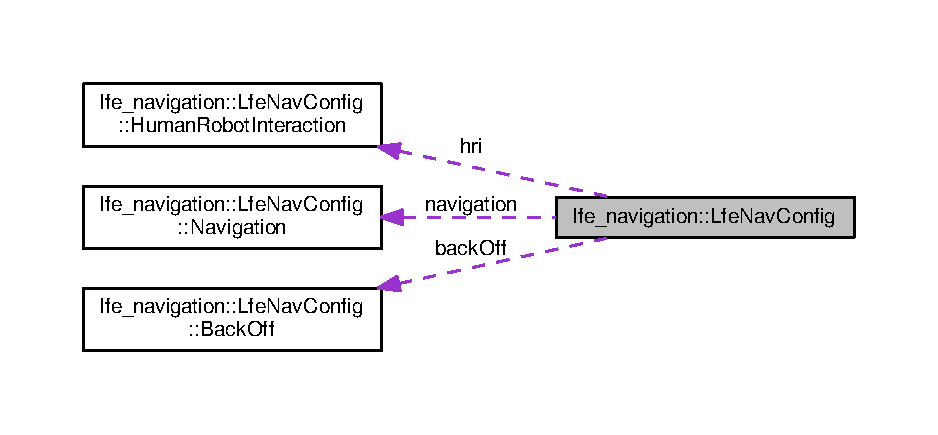
\includegraphics[width=350pt]{classlfe__navigation_1_1LfeNavConfig__coll__graph}
\end{center}
\end{figure}
\subsection*{Classes}
\begin{DoxyCompactItemize}
\item 
struct \hyperlink{structlfe__navigation_1_1LfeNavConfig_1_1BackOff}{Back\+Off}
\item 
struct \hyperlink{structlfe__navigation_1_1LfeNavConfig_1_1HumanRobotInteraction}{Human\+Robot\+Interaction}
\item 
struct \hyperlink{structlfe__navigation_1_1LfeNavConfig_1_1Navigation}{Navigation}
\end{DoxyCompactItemize}
\subsection*{Public Member Functions}
\begin{DoxyCompactItemize}
\item 
\hyperlink{classlfe__navigation_1_1LfeNavConfig_af9b952c60d7d4ae10d84ac2f909edcdb}{Lfe\+Nav\+Config} ()
\begin{DoxyCompactList}\small\item\em Construct the \hyperlink{classlfe__navigation_1_1LfeNavConfig}{Lfe\+Nav\+Config} using default values. \end{DoxyCompactList}\item 
void \hyperlink{classlfe__navigation_1_1LfeNavConfig_a05137fe69a2433269ad8912d66d1451a}{load\+Ros\+Param\+From\+Node\+Handle} (const ros\+::\+Node\+Handle \&nh)
\begin{DoxyCompactList}\small\item\em Load parameters from the configuration user interface via nodehandle. \end{DoxyCompactList}\item 
void \hyperlink{classlfe__navigation_1_1LfeNavConfig_ac864482619cd6e9b864f0d7313c2ef70}{reconfigure} (turtlebot2i\+\_\+lfe\+\_\+navigation\+::\+Lfe\+Nav\+Reconfigure\+Config \&cfg)
\begin{DoxyCompactList}\small\item\em Reconfigure parameters from the dynamic\+\_\+reconfigure config. Change parameters dynamically (e.\+g. with {\ttfamily rosrun rqt\+\_\+reconfigure rqt\+\_\+reconfigure}). A reconfigure server needs to be instantiated that calls this method in it\textquotesingle{}s callback. In case of the package {\itshape lfe\+\_\+navigation} default values are defined in {\itshape P\+R\+O\+J\+E\+C\+T\+\_\+\+S\+R\+C/cfg/\+Lfe\+Nav\+Reconfigure.\+cfg}. \end{DoxyCompactList}\item 
boost\+::mutex \& \hyperlink{classlfe__navigation_1_1LfeNavConfig_a73965acf1db0ac8392f1afff462ff283}{config\+Mutex} ()\hypertarget{classlfe__navigation_1_1LfeNavConfig_a73965acf1db0ac8392f1afff462ff283}{}\label{classlfe__navigation_1_1LfeNavConfig_a73965acf1db0ac8392f1afff462ff283}

\begin{DoxyCompactList}\small\item\em Return the internal config mutex. \end{DoxyCompactList}\end{DoxyCompactItemize}
\subsection*{Public Attributes}
\begin{DoxyCompactItemize}
\item 
struct \hyperlink{structlfe__navigation_1_1LfeNavConfig_1_1Navigation}{lfe\+\_\+navigation\+::\+Lfe\+Nav\+Config\+::\+Navigation} \hyperlink{classlfe__navigation_1_1LfeNavConfig_adaabd1b3bbbb979a70ba2d7e206982a5}{navigation}\hypertarget{classlfe__navigation_1_1LfeNavConfig_adaabd1b3bbbb979a70ba2d7e206982a5}{}\label{classlfe__navigation_1_1LfeNavConfig_adaabd1b3bbbb979a70ba2d7e206982a5}

\begin{DoxyCompactList}\small\item\em \hyperlink{structlfe__navigation_1_1LfeNavConfig_1_1Navigation}{Navigation} related parameters. \end{DoxyCompactList}\item 
struct \hyperlink{structlfe__navigation_1_1LfeNavConfig_1_1HumanRobotInteraction}{lfe\+\_\+navigation\+::\+Lfe\+Nav\+Config\+::\+Human\+Robot\+Interaction} \hyperlink{classlfe__navigation_1_1LfeNavConfig_ac58acb47be5599e0b05510d6b06d2e46}{hri}\hypertarget{classlfe__navigation_1_1LfeNavConfig_ac58acb47be5599e0b05510d6b06d2e46}{}\label{classlfe__navigation_1_1LfeNavConfig_ac58acb47be5599e0b05510d6b06d2e46}

\begin{DoxyCompactList}\small\item\em H\+RI related parameters. \end{DoxyCompactList}\item 
struct \hyperlink{structlfe__navigation_1_1LfeNavConfig_1_1BackOff}{lfe\+\_\+navigation\+::\+Lfe\+Nav\+Config\+::\+Back\+Off} \hyperlink{classlfe__navigation_1_1LfeNavConfig_ae11dfc006a6406617cbd9189568c0839}{back\+Off}\hypertarget{classlfe__navigation_1_1LfeNavConfig_ae11dfc006a6406617cbd9189568c0839}{}\label{classlfe__navigation_1_1LfeNavConfig_ae11dfc006a6406617cbd9189568c0839}

\begin{DoxyCompactList}\small\item\em \hyperlink{structlfe__navigation_1_1LfeNavConfig_1_1BackOff}{Back\+Off} related parameters. \end{DoxyCompactList}\end{DoxyCompactItemize}


\subsection{Detailed Description}
The \hyperlink{classlfe__navigation_1_1LfeNavConfig}{Lfe\+Nav\+Config} class is used as a data type for dynamic configurations. 

\subsection{Constructor \& Destructor Documentation}
\index{lfe\+\_\+navigation\+::\+Lfe\+Nav\+Config@{lfe\+\_\+navigation\+::\+Lfe\+Nav\+Config}!Lfe\+Nav\+Config@{Lfe\+Nav\+Config}}
\index{Lfe\+Nav\+Config@{Lfe\+Nav\+Config}!lfe\+\_\+navigation\+::\+Lfe\+Nav\+Config@{lfe\+\_\+navigation\+::\+Lfe\+Nav\+Config}}
\subsubsection[{\texorpdfstring{Lfe\+Nav\+Config()}{LfeNavConfig()}}]{\setlength{\rightskip}{0pt plus 5cm}lfe\+\_\+navigation\+::\+Lfe\+Nav\+Config\+::\+Lfe\+Nav\+Config (
\begin{DoxyParamCaption}
{}
\end{DoxyParamCaption}
)\hspace{0.3cm}{\ttfamily [inline]}}\hypertarget{classlfe__navigation_1_1LfeNavConfig_af9b952c60d7d4ae10d84ac2f909edcdb}{}\label{classlfe__navigation_1_1LfeNavConfig_af9b952c60d7d4ae10d84ac2f909edcdb}


Construct the \hyperlink{classlfe__navigation_1_1LfeNavConfig}{Lfe\+Nav\+Config} using default values. 

\begin{DoxyWarning}{Warning}
If the {\bfseries rosparam} server or/and {\bfseries dynamic\+\_\+reconfigure} (rqt\+\_\+reconfigure) node are used, the default variables will be overwritten\+: ~\newline

\end{DoxyWarning}


\subsection{Member Function Documentation}
\index{lfe\+\_\+navigation\+::\+Lfe\+Nav\+Config@{lfe\+\_\+navigation\+::\+Lfe\+Nav\+Config}!load\+Ros\+Param\+From\+Node\+Handle@{load\+Ros\+Param\+From\+Node\+Handle}}
\index{load\+Ros\+Param\+From\+Node\+Handle@{load\+Ros\+Param\+From\+Node\+Handle}!lfe\+\_\+navigation\+::\+Lfe\+Nav\+Config@{lfe\+\_\+navigation\+::\+Lfe\+Nav\+Config}}
\subsubsection[{\texorpdfstring{load\+Ros\+Param\+From\+Node\+Handle(const ros\+::\+Node\+Handle \&nh)}{loadRosParamFromNodeHandle(const ros::NodeHandle &nh)}}]{\setlength{\rightskip}{0pt plus 5cm}void lfe\+\_\+navigation\+::\+Lfe\+Nav\+Config\+::load\+Ros\+Param\+From\+Node\+Handle (
\begin{DoxyParamCaption}
\item[{const ros\+::\+Node\+Handle \&}]{nh}
\end{DoxyParamCaption}
)}\hypertarget{classlfe__navigation_1_1LfeNavConfig_a05137fe69a2433269ad8912d66d1451a}{}\label{classlfe__navigation_1_1LfeNavConfig_a05137fe69a2433269ad8912d66d1451a}


Load parameters from the configuration user interface via nodehandle. 


\begin{DoxyParams}{Parameters}
{\em nh} & const reference to the local ros\+::\+Node\+Handle \\
\hline
\end{DoxyParams}
\index{lfe\+\_\+navigation\+::\+Lfe\+Nav\+Config@{lfe\+\_\+navigation\+::\+Lfe\+Nav\+Config}!reconfigure@{reconfigure}}
\index{reconfigure@{reconfigure}!lfe\+\_\+navigation\+::\+Lfe\+Nav\+Config@{lfe\+\_\+navigation\+::\+Lfe\+Nav\+Config}}
\subsubsection[{\texorpdfstring{reconfigure(turtlebot2i\+\_\+lfe\+\_\+navigation\+::\+Lfe\+Nav\+Reconfigure\+Config \&cfg)}{reconfigure(turtlebot2i_lfe_navigation::LfeNavReconfigureConfig &cfg)}}]{\setlength{\rightskip}{0pt plus 5cm}void lfe\+\_\+navigation\+::\+Lfe\+Nav\+Config\+::reconfigure (
\begin{DoxyParamCaption}
\item[{turtlebot2i\+\_\+lfe\+\_\+navigation\+::\+Lfe\+Nav\+Reconfigure\+Config \&}]{cfg}
\end{DoxyParamCaption}
)}\hypertarget{classlfe__navigation_1_1LfeNavConfig_ac864482619cd6e9b864f0d7313c2ef70}{}\label{classlfe__navigation_1_1LfeNavConfig_ac864482619cd6e9b864f0d7313c2ef70}


Reconfigure parameters from the dynamic\+\_\+reconfigure config. Change parameters dynamically (e.\+g. with {\ttfamily rosrun rqt\+\_\+reconfigure rqt\+\_\+reconfigure}). A reconfigure server needs to be instantiated that calls this method in it\textquotesingle{}s callback. In case of the package {\itshape lfe\+\_\+navigation} default values are defined in {\itshape P\+R\+O\+J\+E\+C\+T\+\_\+\+S\+R\+C/cfg/\+Lfe\+Nav\+Reconfigure.\+cfg}. 


\begin{DoxyParams}{Parameters}
{\em cfg} & Config class autogenerated by dynamic\+\_\+reconfigure according to the cfg-\/file mentioned above. \\
\hline
\end{DoxyParams}


The documentation for this class was generated from the following file\+:\begin{DoxyCompactItemize}
\item 
lfe\+\_\+nav\+\_\+config.\+h\end{DoxyCompactItemize}

\hypertarget{classlfe__navigation_1_1LfeNavLogger}{}\section{lfe\+\_\+navigation\+:\+:Lfe\+Nav\+Logger Class Reference}
\label{classlfe__navigation_1_1LfeNavLogger}\index{lfe\+\_\+navigation\+::\+Lfe\+Nav\+Logger@{lfe\+\_\+navigation\+::\+Lfe\+Nav\+Logger}}


The \hyperlink{classlfe__navigation_1_1LfeNavLogger}{Lfe\+Nav\+Logger} is responsible for parameter logging and publishing of log data as messages.  




{\ttfamily \#include $<$lfe\+\_\+nav\+\_\+logger.\+h$>$}

\subsection*{Public Member Functions}
\begin{DoxyCompactItemize}
\item 
\hyperlink{classlfe__navigation_1_1LfeNavLogger_a69c8bb8c1ffa217d452ebfce0fe01830}{Lfe\+Nav\+Logger} (ros\+::\+Node\+Handle \&nh)
\begin{DoxyCompactList}\small\item\em Overloaded constructor that takes in a nodehandle. \end{DoxyCompactList}\item 
void \hyperlink{classlfe__navigation_1_1LfeNavLogger_adca0a164d19d1d6fe5cfd9f8971c1789}{bo\+\_\+log\+\_\+init} (double back\+\_\+velocity, double back\+\_\+duration, int wait\+\_\+duration, std\+::vector$<$ double $>$ human\+\_\+dist\+\_\+seq, std\+::vector$<$ double $>$ human\+\_\+dist\+\_\+time\+\_\+seq, double human\+\_\+approach\+\_\+vel, double robot\+\_\+vel, std\+::string frame\+\_\+id)
\begin{DoxyCompactList}\small\item\em Overloaded method to initialize a back-\/off log message in a frontal path-\/crossing situation. \end{DoxyCompactList}\item 
void \hyperlink{classlfe__navigation_1_1LfeNavLogger_a39d9b5ec6adc8b0e9f2a4231e6bc42d7}{st\+\_\+log\+\_\+init} (int wait\+\_\+duration, std\+::vector$<$ double $>$ human\+\_\+dist\+\_\+seq, std\+::vector$<$ double $>$ human\+\_\+dist\+\_\+time\+\_\+seq, double human\+\_\+approach\+\_\+vel, double robot\+\_\+vel, std\+::string frame\+\_\+id)
\begin{DoxyCompactList}\small\item\em Overloaded method to initialize a stop motion cue log message in a frontal path-\/crossing situation. \end{DoxyCompactList}\item 
void \hyperlink{classlfe__navigation_1_1LfeNavLogger_a4354882dc26d1d1a2d54cae0c103819d}{bo\+\_\+log\+\_\+init} (double back\+\_\+velocity, double back\+\_\+duration, int wait\+\_\+duration, double robot\+\_\+vel, std\+::string frame\+\_\+id)
\begin{DoxyCompactList}\small\item\em Overloaded method to initialize a back-\/off log message in a lateral path-\/crossing situation. \end{DoxyCompactList}\item 
void \hyperlink{classlfe__navigation_1_1LfeNavLogger_aa33f5443f3ef9967303434786bdad551}{st\+\_\+log\+\_\+init} (int wait\+\_\+duration, double robot\+\_\+vel, std\+::string frame\+\_\+id)
\begin{DoxyCompactList}\small\item\em Overloaded method to initialize a stop motion cue log message in a lateral path-\/crossing situation. \end{DoxyCompactList}\item 
void \hyperlink{classlfe__navigation_1_1LfeNavLogger_a1496e394cd69320d480dd30d0c66b319}{finalize\+\_\+log} (bool back\+\_\+off, std\+::vector$<$ double $>$ human\+\_\+mc\+\_\+dist\+\_\+seq, std\+::vector$<$ double $>$ human\+\_\+mc\+\_\+dist\+\_\+time\+\_\+seq, bool human\+\_\+continue\+\_\+goal)
\begin{DoxyCompactList}\small\item\em Method finalizing the logging of both, back-\/off and stop motion cue, and publishing it as a message. \end{DoxyCompactList}\end{DoxyCompactItemize}


\subsection{Detailed Description}
The \hyperlink{classlfe__navigation_1_1LfeNavLogger}{Lfe\+Nav\+Logger} is responsible for parameter logging and publishing of log data as messages. 

Methods of the \hyperlink{classlfe__navigation_1_1LfeNavLogger}{Lfe\+Nav\+Logger} are called by the \hyperlink{classlfe__navigation_1_1DynamicObstacleListener}{Dynamic\+Obstacle\+Listener} to initialize or finalize a logging message. Logging messages are published and can be recorded into bagfiles. 

\subsection{Constructor \& Destructor Documentation}
\index{lfe\+\_\+navigation\+::\+Lfe\+Nav\+Logger@{lfe\+\_\+navigation\+::\+Lfe\+Nav\+Logger}!Lfe\+Nav\+Logger@{Lfe\+Nav\+Logger}}
\index{Lfe\+Nav\+Logger@{Lfe\+Nav\+Logger}!lfe\+\_\+navigation\+::\+Lfe\+Nav\+Logger@{lfe\+\_\+navigation\+::\+Lfe\+Nav\+Logger}}
\subsubsection[{\texorpdfstring{Lfe\+Nav\+Logger(ros\+::\+Node\+Handle \&nh)}{LfeNavLogger(ros::NodeHandle &nh)}}]{\setlength{\rightskip}{0pt plus 5cm}lfe\+\_\+navigation\+::\+Lfe\+Nav\+Logger\+::\+Lfe\+Nav\+Logger (
\begin{DoxyParamCaption}
\item[{ros\+::\+Node\+Handle \&}]{nh}
\end{DoxyParamCaption}
)}\hypertarget{classlfe__navigation_1_1LfeNavLogger_a69c8bb8c1ffa217d452ebfce0fe01830}{}\label{classlfe__navigation_1_1LfeNavLogger_a69c8bb8c1ffa217d452ebfce0fe01830}


Overloaded constructor that takes in a nodehandle. 


\begin{DoxyParams}{Parameters}
{\em nh} & The nodehandle by which logging messages are published \\
\hline
\end{DoxyParams}


\subsection{Member Function Documentation}
\index{lfe\+\_\+navigation\+::\+Lfe\+Nav\+Logger@{lfe\+\_\+navigation\+::\+Lfe\+Nav\+Logger}!bo\+\_\+log\+\_\+init@{bo\+\_\+log\+\_\+init}}
\index{bo\+\_\+log\+\_\+init@{bo\+\_\+log\+\_\+init}!lfe\+\_\+navigation\+::\+Lfe\+Nav\+Logger@{lfe\+\_\+navigation\+::\+Lfe\+Nav\+Logger}}
\subsubsection[{\texorpdfstring{bo\+\_\+log\+\_\+init(double back\+\_\+velocity, double back\+\_\+duration, int wait\+\_\+duration, std\+::vector$<$ double $>$ human\+\_\+dist\+\_\+seq, std\+::vector$<$ double $>$ human\+\_\+dist\+\_\+time\+\_\+seq, double human\+\_\+approach\+\_\+vel, double robot\+\_\+vel, std\+::string frame\+\_\+id)}{bo_log_init(double back_velocity, double back_duration, int wait_duration, std::vector< double > human_dist_seq, std::vector< double > human_dist_time_seq, double human_approach_vel, double robot_vel, std::string frame_id)}}]{\setlength{\rightskip}{0pt plus 5cm}void lfe\+\_\+navigation\+::\+Lfe\+Nav\+Logger\+::bo\+\_\+log\+\_\+init (
\begin{DoxyParamCaption}
\item[{double}]{back\+\_\+velocity, }
\item[{double}]{back\+\_\+duration, }
\item[{int}]{wait\+\_\+duration, }
\item[{std\+::vector$<$ double $>$}]{human\+\_\+dist\+\_\+seq, }
\item[{std\+::vector$<$ double $>$}]{human\+\_\+dist\+\_\+time\+\_\+seq, }
\item[{double}]{human\+\_\+approach\+\_\+vel, }
\item[{double}]{robot\+\_\+vel, }
\item[{std\+::string}]{frame\+\_\+id}
\end{DoxyParamCaption}
)}\hypertarget{classlfe__navigation_1_1LfeNavLogger_adca0a164d19d1d6fe5cfd9f8971c1789}{}\label{classlfe__navigation_1_1LfeNavLogger_adca0a164d19d1d6fe5cfd9f8971c1789}


Overloaded method to initialize a back-\/off log message in a frontal path-\/crossing situation. 


\begin{DoxyParams}{Parameters}
{\em back\+\_\+velocity} & Configured back-\/off backwards velocity \\
\hline
{\em back\+\_\+duration} & Configured duration of the back-\/off \\
\hline
{\em wait\+\_\+duration} & Configured duration to wait before navigation is continued \\
\hline
{\em human\+\_\+dist\+\_\+seq} & Stores the distances of the approaching human \\
\hline
{\em human\+\_\+dist\+\_\+time\+\_\+seq} & Stores the timestamp of the distances in human\+\_\+dist\+\_\+seq \\
\hline
{\em human\+\_\+approach\+\_\+vel} & Stores the approaching velocity of the human \\
\hline
{\em robot\+\_\+vel} & Current robot velocity \\
\hline
{\em frame\+\_\+id} & Frame id of the image, from which the back-\/off was triggered \\
\hline
\end{DoxyParams}
\index{lfe\+\_\+navigation\+::\+Lfe\+Nav\+Logger@{lfe\+\_\+navigation\+::\+Lfe\+Nav\+Logger}!bo\+\_\+log\+\_\+init@{bo\+\_\+log\+\_\+init}}
\index{bo\+\_\+log\+\_\+init@{bo\+\_\+log\+\_\+init}!lfe\+\_\+navigation\+::\+Lfe\+Nav\+Logger@{lfe\+\_\+navigation\+::\+Lfe\+Nav\+Logger}}
\subsubsection[{\texorpdfstring{bo\+\_\+log\+\_\+init(double back\+\_\+velocity, double back\+\_\+duration, int wait\+\_\+duration, double robot\+\_\+vel, std\+::string frame\+\_\+id)}{bo_log_init(double back_velocity, double back_duration, int wait_duration, double robot_vel, std::string frame_id)}}]{\setlength{\rightskip}{0pt plus 5cm}void lfe\+\_\+navigation\+::\+Lfe\+Nav\+Logger\+::bo\+\_\+log\+\_\+init (
\begin{DoxyParamCaption}
\item[{double}]{back\+\_\+velocity, }
\item[{double}]{back\+\_\+duration, }
\item[{int}]{wait\+\_\+duration, }
\item[{double}]{robot\+\_\+vel, }
\item[{std\+::string}]{frame\+\_\+id}
\end{DoxyParamCaption}
)}\hypertarget{classlfe__navigation_1_1LfeNavLogger_a4354882dc26d1d1a2d54cae0c103819d}{}\label{classlfe__navigation_1_1LfeNavLogger_a4354882dc26d1d1a2d54cae0c103819d}


Overloaded method to initialize a back-\/off log message in a lateral path-\/crossing situation. 


\begin{DoxyParams}{Parameters}
{\em back\+\_\+velocity} & Configured back-\/off backwards velocity \\
\hline
{\em back\+\_\+duration} & Configured duration of the back-\/off \\
\hline
{\em wait\+\_\+duration} & Configured duration to wait before navigation is continued \\
\hline
{\em robot\+\_\+vel} & Current robot velocity \\
\hline
{\em frame\+\_\+id} & Frame id of the image, from which the back-\/off was triggered \\
\hline
\end{DoxyParams}
\index{lfe\+\_\+navigation\+::\+Lfe\+Nav\+Logger@{lfe\+\_\+navigation\+::\+Lfe\+Nav\+Logger}!finalize\+\_\+log@{finalize\+\_\+log}}
\index{finalize\+\_\+log@{finalize\+\_\+log}!lfe\+\_\+navigation\+::\+Lfe\+Nav\+Logger@{lfe\+\_\+navigation\+::\+Lfe\+Nav\+Logger}}
\subsubsection[{\texorpdfstring{finalize\+\_\+log(bool back\+\_\+off, std\+::vector$<$ double $>$ human\+\_\+mc\+\_\+dist\+\_\+seq, std\+::vector$<$ double $>$ human\+\_\+mc\+\_\+dist\+\_\+time\+\_\+seq, bool human\+\_\+continue\+\_\+goal)}{finalize_log(bool back_off, std::vector< double > human_mc_dist_seq, std::vector< double > human_mc_dist_time_seq, bool human_continue_goal)}}]{\setlength{\rightskip}{0pt plus 5cm}void lfe\+\_\+navigation\+::\+Lfe\+Nav\+Logger\+::finalize\+\_\+log (
\begin{DoxyParamCaption}
\item[{bool}]{back\+\_\+off, }
\item[{std\+::vector$<$ double $>$}]{human\+\_\+mc\+\_\+dist\+\_\+seq, }
\item[{std\+::vector$<$ double $>$}]{human\+\_\+mc\+\_\+dist\+\_\+time\+\_\+seq, }
\item[{bool}]{human\+\_\+continue\+\_\+goal}
\end{DoxyParamCaption}
)}\hypertarget{classlfe__navigation_1_1LfeNavLogger_a1496e394cd69320d480dd30d0c66b319}{}\label{classlfe__navigation_1_1LfeNavLogger_a1496e394cd69320d480dd30d0c66b319}


Method finalizing the logging of both, back-\/off and stop motion cue, and publishing it as a message. 


\begin{DoxyParams}{Parameters}
{\em back\+\_\+off} & True, if motion cue is back-\/off, False, if motion cue is stop \\
\hline
{\em human\+\_\+mc\+\_\+dist\+\_\+seq} & Stores the distances of the human during the motion cue execution \\
\hline
{\em human\+\_\+mc\+\_\+dist\+\_\+time\+\_\+seq} & Stores the time stamps of the distances in the humanh\+\_\+mc\+\_\+dist\+\_\+seq array \\
\hline
{\em human\+\_\+continue\+\_\+goal} & True, if a human was still detected while continuing the navigation \\
\hline
\end{DoxyParams}
\index{lfe\+\_\+navigation\+::\+Lfe\+Nav\+Logger@{lfe\+\_\+navigation\+::\+Lfe\+Nav\+Logger}!st\+\_\+log\+\_\+init@{st\+\_\+log\+\_\+init}}
\index{st\+\_\+log\+\_\+init@{st\+\_\+log\+\_\+init}!lfe\+\_\+navigation\+::\+Lfe\+Nav\+Logger@{lfe\+\_\+navigation\+::\+Lfe\+Nav\+Logger}}
\subsubsection[{\texorpdfstring{st\+\_\+log\+\_\+init(int wait\+\_\+duration, std\+::vector$<$ double $>$ human\+\_\+dist\+\_\+seq, std\+::vector$<$ double $>$ human\+\_\+dist\+\_\+time\+\_\+seq, double human\+\_\+approach\+\_\+vel, double robot\+\_\+vel, std\+::string frame\+\_\+id)}{st_log_init(int wait_duration, std::vector< double > human_dist_seq, std::vector< double > human_dist_time_seq, double human_approach_vel, double robot_vel, std::string frame_id)}}]{\setlength{\rightskip}{0pt plus 5cm}void lfe\+\_\+navigation\+::\+Lfe\+Nav\+Logger\+::st\+\_\+log\+\_\+init (
\begin{DoxyParamCaption}
\item[{int}]{wait\+\_\+duration, }
\item[{std\+::vector$<$ double $>$}]{human\+\_\+dist\+\_\+seq, }
\item[{std\+::vector$<$ double $>$}]{human\+\_\+dist\+\_\+time\+\_\+seq, }
\item[{double}]{human\+\_\+approach\+\_\+vel, }
\item[{double}]{robot\+\_\+vel, }
\item[{std\+::string}]{frame\+\_\+id}
\end{DoxyParamCaption}
)}\hypertarget{classlfe__navigation_1_1LfeNavLogger_a39d9b5ec6adc8b0e9f2a4231e6bc42d7}{}\label{classlfe__navigation_1_1LfeNavLogger_a39d9b5ec6adc8b0e9f2a4231e6bc42d7}


Overloaded method to initialize a stop motion cue log message in a frontal path-\/crossing situation. 


\begin{DoxyParams}{Parameters}
{\em wait\+\_\+duration} & Configured duration to wait before navigation is continued \\
\hline
{\em human\+\_\+dist\+\_\+seq} & Stores the distances of the approaching human \\
\hline
{\em human\+\_\+dist\+\_\+time\+\_\+seq} & Stores the timestamp of the distances in human\+\_\+dist\+\_\+seq \\
\hline
{\em human\+\_\+approach\+\_\+vel} & Stores the approaching velocity of the human \\
\hline
{\em robot\+\_\+vel} & Current robot velocity \\
\hline
{\em frame\+\_\+id} & Frame id of the image, from which the back-\/off was triggered \\
\hline
\end{DoxyParams}
\index{lfe\+\_\+navigation\+::\+Lfe\+Nav\+Logger@{lfe\+\_\+navigation\+::\+Lfe\+Nav\+Logger}!st\+\_\+log\+\_\+init@{st\+\_\+log\+\_\+init}}
\index{st\+\_\+log\+\_\+init@{st\+\_\+log\+\_\+init}!lfe\+\_\+navigation\+::\+Lfe\+Nav\+Logger@{lfe\+\_\+navigation\+::\+Lfe\+Nav\+Logger}}
\subsubsection[{\texorpdfstring{st\+\_\+log\+\_\+init(int wait\+\_\+duration, double robot\+\_\+vel, std\+::string frame\+\_\+id)}{st_log_init(int wait_duration, double robot_vel, std::string frame_id)}}]{\setlength{\rightskip}{0pt plus 5cm}void lfe\+\_\+navigation\+::\+Lfe\+Nav\+Logger\+::st\+\_\+log\+\_\+init (
\begin{DoxyParamCaption}
\item[{int}]{wait\+\_\+duration, }
\item[{double}]{robot\+\_\+vel, }
\item[{std\+::string}]{frame\+\_\+id}
\end{DoxyParamCaption}
)}\hypertarget{classlfe__navigation_1_1LfeNavLogger_aa33f5443f3ef9967303434786bdad551}{}\label{classlfe__navigation_1_1LfeNavLogger_aa33f5443f3ef9967303434786bdad551}


Overloaded method to initialize a stop motion cue log message in a lateral path-\/crossing situation. 


\begin{DoxyParams}{Parameters}
{\em wait\+\_\+duration} & Configured duration to wait before navigation is continued \\
\hline
{\em robot\+\_\+vel} & Current robot velocity \\
\hline
{\em frame\+\_\+id} & Frame id of the image, from which the back-\/off was triggered \\
\hline
\end{DoxyParams}


The documentation for this class was generated from the following file\+:\begin{DoxyCompactItemize}
\item 
lfe\+\_\+nav\+\_\+logger.\+h\end{DoxyCompactItemize}

\hypertarget{structlfe__navigation_1_1LfeNavConfig_1_1Navigation}{}\section{lfe\+\_\+navigation\+:\+:Lfe\+Nav\+Config\+:\+:Navigation Struct Reference}
\label{structlfe__navigation_1_1LfeNavConfig_1_1Navigation}\index{lfe\+\_\+navigation\+::\+Lfe\+Nav\+Config\+::\+Navigation@{lfe\+\_\+navigation\+::\+Lfe\+Nav\+Config\+::\+Navigation}}
\subsection*{Public Attributes}
\begin{DoxyCompactItemize}
\item 
double \hyperlink{structlfe__navigation_1_1LfeNavConfig_1_1Navigation_abb022bddb3449194fca51d520664bf0e}{goal1\+\_\+pos\+\_\+x}\hypertarget{structlfe__navigation_1_1LfeNavConfig_1_1Navigation_abb022bddb3449194fca51d520664bf0e}{}\label{structlfe__navigation_1_1LfeNavConfig_1_1Navigation_abb022bddb3449194fca51d520664bf0e}

\begin{DoxyCompactList}\small\item\em x coordinate of goal1 position \end{DoxyCompactList}\item 
double \hyperlink{structlfe__navigation_1_1LfeNavConfig_1_1Navigation_a466cfb8a9e82f36785e7309ea1e31829}{goal1\+\_\+pos\+\_\+y}\hypertarget{structlfe__navigation_1_1LfeNavConfig_1_1Navigation_a466cfb8a9e82f36785e7309ea1e31829}{}\label{structlfe__navigation_1_1LfeNavConfig_1_1Navigation_a466cfb8a9e82f36785e7309ea1e31829}

\begin{DoxyCompactList}\small\item\em y coordinate of goal1 position \end{DoxyCompactList}\item 
double \hyperlink{structlfe__navigation_1_1LfeNavConfig_1_1Navigation_ad2a692b49b6ac9e0684f4f146da99779}{goal1\+\_\+pos\+\_\+z}\hypertarget{structlfe__navigation_1_1LfeNavConfig_1_1Navigation_ad2a692b49b6ac9e0684f4f146da99779}{}\label{structlfe__navigation_1_1LfeNavConfig_1_1Navigation_ad2a692b49b6ac9e0684f4f146da99779}

\begin{DoxyCompactList}\small\item\em z coordinate of goal1 position \end{DoxyCompactList}\item 
double \hyperlink{structlfe__navigation_1_1LfeNavConfig_1_1Navigation_a7b7b4ab4f9981d66e81edc07d497ef3e}{goal1\+\_\+orientation}\hypertarget{structlfe__navigation_1_1LfeNavConfig_1_1Navigation_a7b7b4ab4f9981d66e81edc07d497ef3e}{}\label{structlfe__navigation_1_1LfeNavConfig_1_1Navigation_a7b7b4ab4f9981d66e81edc07d497ef3e}

\begin{DoxyCompactList}\small\item\em goal1 orientation as radian for z axis \end{DoxyCompactList}\item 
double \hyperlink{structlfe__navigation_1_1LfeNavConfig_1_1Navigation_af029a9f57dda1580b7124269a7eed505}{goal2\+\_\+pos\+\_\+x}\hypertarget{structlfe__navigation_1_1LfeNavConfig_1_1Navigation_af029a9f57dda1580b7124269a7eed505}{}\label{structlfe__navigation_1_1LfeNavConfig_1_1Navigation_af029a9f57dda1580b7124269a7eed505}

\begin{DoxyCompactList}\small\item\em x coordinate of goal2 position \end{DoxyCompactList}\item 
double \hyperlink{structlfe__navigation_1_1LfeNavConfig_1_1Navigation_a5a3e8e6e9d21288a51e4196f3c6e08f1}{goal2\+\_\+pos\+\_\+y}\hypertarget{structlfe__navigation_1_1LfeNavConfig_1_1Navigation_a5a3e8e6e9d21288a51e4196f3c6e08f1}{}\label{structlfe__navigation_1_1LfeNavConfig_1_1Navigation_a5a3e8e6e9d21288a51e4196f3c6e08f1}

\begin{DoxyCompactList}\small\item\em y coordinate of goal2 position \end{DoxyCompactList}\item 
double \hyperlink{structlfe__navigation_1_1LfeNavConfig_1_1Navigation_a489c47336774dacd345cf390ed689cf9}{goal2\+\_\+pos\+\_\+z}\hypertarget{structlfe__navigation_1_1LfeNavConfig_1_1Navigation_a489c47336774dacd345cf390ed689cf9}{}\label{structlfe__navigation_1_1LfeNavConfig_1_1Navigation_a489c47336774dacd345cf390ed689cf9}

\begin{DoxyCompactList}\small\item\em z coordinate of goal2 position \end{DoxyCompactList}\item 
double \hyperlink{structlfe__navigation_1_1LfeNavConfig_1_1Navigation_a111b9dc683915a5d3327a33ad943e18d}{goal2\+\_\+orientation}\hypertarget{structlfe__navigation_1_1LfeNavConfig_1_1Navigation_a111b9dc683915a5d3327a33ad943e18d}{}\label{structlfe__navigation_1_1LfeNavConfig_1_1Navigation_a111b9dc683915a5d3327a33ad943e18d}

\begin{DoxyCompactList}\small\item\em goal2 orientation as radian for z axis \end{DoxyCompactList}\item 
double \hyperlink{structlfe__navigation_1_1LfeNavConfig_1_1Navigation_ab52669cc577e7f03fcaab25cfb83e2a2}{goal3\+\_\+pos\+\_\+x}\hypertarget{structlfe__navigation_1_1LfeNavConfig_1_1Navigation_ab52669cc577e7f03fcaab25cfb83e2a2}{}\label{structlfe__navigation_1_1LfeNavConfig_1_1Navigation_ab52669cc577e7f03fcaab25cfb83e2a2}

\begin{DoxyCompactList}\small\item\em x coordinate of goal3 position \end{DoxyCompactList}\item 
double \hyperlink{structlfe__navigation_1_1LfeNavConfig_1_1Navigation_a37e831281f17149b912a9e544c8f47b2}{goal3\+\_\+pos\+\_\+y}\hypertarget{structlfe__navigation_1_1LfeNavConfig_1_1Navigation_a37e831281f17149b912a9e544c8f47b2}{}\label{structlfe__navigation_1_1LfeNavConfig_1_1Navigation_a37e831281f17149b912a9e544c8f47b2}

\begin{DoxyCompactList}\small\item\em y coordinate of goal3 position \end{DoxyCompactList}\item 
double \hyperlink{structlfe__navigation_1_1LfeNavConfig_1_1Navigation_a11c2e0e0dcf592311ad115c85cffb33d}{goal3\+\_\+pos\+\_\+z}\hypertarget{structlfe__navigation_1_1LfeNavConfig_1_1Navigation_a11c2e0e0dcf592311ad115c85cffb33d}{}\label{structlfe__navigation_1_1LfeNavConfig_1_1Navigation_a11c2e0e0dcf592311ad115c85cffb33d}

\begin{DoxyCompactList}\small\item\em z coordinate of goal3 position \end{DoxyCompactList}\item 
double \hyperlink{structlfe__navigation_1_1LfeNavConfig_1_1Navigation_a983e0a1daa2aceae55047d3b67691475}{goal3\+\_\+orientation}\hypertarget{structlfe__navigation_1_1LfeNavConfig_1_1Navigation_a983e0a1daa2aceae55047d3b67691475}{}\label{structlfe__navigation_1_1LfeNavConfig_1_1Navigation_a983e0a1daa2aceae55047d3b67691475}

\begin{DoxyCompactList}\small\item\em goal3 orientation as radian for z axis \end{DoxyCompactList}\end{DoxyCompactItemize}


The documentation for this struct was generated from the following file\+:\begin{DoxyCompactItemize}
\item 
lfe\+\_\+nav\+\_\+config.\+h\end{DoxyCompactItemize}

\hypertarget{classlfe__navigation_1_1NavigationManager}{}\section{lfe\+\_\+navigation\+:\+:Navigation\+Manager Class Reference}
\label{classlfe__navigation_1_1NavigationManager}\index{lfe\+\_\+navigation\+::\+Navigation\+Manager@{lfe\+\_\+navigation\+::\+Navigation\+Manager}}


The \hyperlink{classlfe__navigation_1_1NavigationManager}{Navigation\+Manager} contains all methods responsible for navigation.  




{\ttfamily \#include $<$navigation\+\_\+manager.\+h$>$}

\subsection*{Public Member Functions}
\begin{DoxyCompactItemize}
\item 
\hyperlink{classlfe__navigation_1_1NavigationManager_a04357660f9d9c640eb3aefc382def800}{Navigation\+Manager} (ros\+::\+Node\+Handle \&nh)
\begin{DoxyCompactList}\small\item\em Overloaded constructor that takes in a nodehandle. \end{DoxyCompactList}\item 
void \hyperlink{classlfe__navigation_1_1NavigationManager_a708b61e1da4997d9e52dba82ce8abdb9}{send\+Goal} ()\hypertarget{classlfe__navigation_1_1NavigationManager_a708b61e1da4997d9e52dba82ce8abdb9}{}\label{classlfe__navigation_1_1NavigationManager_a708b61e1da4997d9e52dba82ce8abdb9}

\begin{DoxyCompactList}\small\item\em Method sending goals to the actionlib server. \end{DoxyCompactList}\item 
void \hyperlink{classlfe__navigation_1_1NavigationManager_a8a263bf41e271138c7827c4dd5ab85fa}{stop\+Goal} ()\hypertarget{classlfe__navigation_1_1NavigationManager_a8a263bf41e271138c7827c4dd5ab85fa}{}\label{classlfe__navigation_1_1NavigationManager_a8a263bf41e271138c7827c4dd5ab85fa}

\begin{DoxyCompactList}\small\item\em Method setting paused\+\_\+ to true. Paused\+\_\+ stops the navigation in \hyperlink{classlfe__navigation_1_1NavigationManager_a708b61e1da4997d9e52dba82ce8abdb9}{send\+Goal()} method. \end{DoxyCompactList}\item 
void \hyperlink{classlfe__navigation_1_1NavigationManager_ac779f9a9e239b22a3c3442f4fccafced}{back\+Off} (double back\+\_\+velocity, double back\+\_\+seconds)
\begin{DoxyCompactList}\small\item\em Method executing the back-\/off motion cue. \end{DoxyCompactList}\item 
void \hyperlink{classlfe__navigation_1_1NavigationManager_a52d2f66551c0537ee109013bb0a4fb06}{continue\+Goal} (int seconds)
\begin{DoxyCompactList}\small\item\em Method Setting sending\+Goal\+\_\+ to true to continue the navigation. \end{DoxyCompactList}\item 
void \hyperlink{classlfe__navigation_1_1NavigationManager_a6294d8559a40febde615c1d91e79a6ff}{set\+Goal1} (double x, double y, double z, double orientation)
\begin{DoxyCompactList}\small\item\em Method setting new coordinates to goal1\+\_\+ variable. \end{DoxyCompactList}\item 
void \hyperlink{classlfe__navigation_1_1NavigationManager_add3a6bd2acafa6f4ac950d71603bd97e}{set\+Goal2} (double x, double y, double z, double orientation)
\begin{DoxyCompactList}\small\item\em Method setting new coordinates to goal2\+\_\+ variable. \end{DoxyCompactList}\item 
void \hyperlink{classlfe__navigation_1_1NavigationManager_a8a751145c42018976caf845a64c8f6ea}{set\+Goal3} (double x, double y, double z, double orientation)
\begin{DoxyCompactList}\small\item\em Method setting new coordinates to goal3\+\_\+ variable. \end{DoxyCompactList}\end{DoxyCompactItemize}


\subsection{Detailed Description}
The \hyperlink{classlfe__navigation_1_1NavigationManager}{Navigation\+Manager} contains all methods responsible for navigation. 

The \hyperlink{classlfe__navigation_1_1NavigationManager}{Navigation\+Manager} class manages the communication with the action\+Lib server and executes the motion cues. It is responsible to start, cancel and continue a navigation goal. 

\subsection{Constructor \& Destructor Documentation}
\index{lfe\+\_\+navigation\+::\+Navigation\+Manager@{lfe\+\_\+navigation\+::\+Navigation\+Manager}!Navigation\+Manager@{Navigation\+Manager}}
\index{Navigation\+Manager@{Navigation\+Manager}!lfe\+\_\+navigation\+::\+Navigation\+Manager@{lfe\+\_\+navigation\+::\+Navigation\+Manager}}
\subsubsection[{\texorpdfstring{Navigation\+Manager(ros\+::\+Node\+Handle \&nh)}{NavigationManager(ros::NodeHandle &nh)}}]{\setlength{\rightskip}{0pt plus 5cm}lfe\+\_\+navigation\+::\+Navigation\+Manager\+::\+Navigation\+Manager (
\begin{DoxyParamCaption}
\item[{ros\+::\+Node\+Handle \&}]{nh}
\end{DoxyParamCaption}
)}\hypertarget{classlfe__navigation_1_1NavigationManager_a04357660f9d9c640eb3aefc382def800}{}\label{classlfe__navigation_1_1NavigationManager_a04357660f9d9c640eb3aefc382def800}


Overloaded constructor that takes in a nodehandle. 


\begin{DoxyParams}{Parameters}
{\em nh} & The nodehandle by which back-\/off backwards velocity is published for wheel control \\
\hline
\end{DoxyParams}


\subsection{Member Function Documentation}
\index{lfe\+\_\+navigation\+::\+Navigation\+Manager@{lfe\+\_\+navigation\+::\+Navigation\+Manager}!back\+Off@{back\+Off}}
\index{back\+Off@{back\+Off}!lfe\+\_\+navigation\+::\+Navigation\+Manager@{lfe\+\_\+navigation\+::\+Navigation\+Manager}}
\subsubsection[{\texorpdfstring{back\+Off(double back\+\_\+velocity, double back\+\_\+seconds)}{backOff(double back_velocity, double back_seconds)}}]{\setlength{\rightskip}{0pt plus 5cm}void lfe\+\_\+navigation\+::\+Navigation\+Manager\+::back\+Off (
\begin{DoxyParamCaption}
\item[{double}]{back\+\_\+velocity, }
\item[{double}]{back\+\_\+seconds}
\end{DoxyParamCaption}
)}\hypertarget{classlfe__navigation_1_1NavigationManager_ac779f9a9e239b22a3c3442f4fccafced}{}\label{classlfe__navigation_1_1NavigationManager_ac779f9a9e239b22a3c3442f4fccafced}


Method executing the back-\/off motion cue. 


\begin{DoxyParams}{Parameters}
{\em back\+\_\+velocity} & Backwards velocity \\
\hline
{\em back\+\_\+seconds} & Back-\/off duration in seconds \\
\hline
\end{DoxyParams}
\index{lfe\+\_\+navigation\+::\+Navigation\+Manager@{lfe\+\_\+navigation\+::\+Navigation\+Manager}!continue\+Goal@{continue\+Goal}}
\index{continue\+Goal@{continue\+Goal}!lfe\+\_\+navigation\+::\+Navigation\+Manager@{lfe\+\_\+navigation\+::\+Navigation\+Manager}}
\subsubsection[{\texorpdfstring{continue\+Goal(int seconds)}{continueGoal(int seconds)}}]{\setlength{\rightskip}{0pt plus 5cm}void lfe\+\_\+navigation\+::\+Navigation\+Manager\+::continue\+Goal (
\begin{DoxyParamCaption}
\item[{int}]{seconds}
\end{DoxyParamCaption}
)}\hypertarget{classlfe__navigation_1_1NavigationManager_a52d2f66551c0537ee109013bb0a4fb06}{}\label{classlfe__navigation_1_1NavigationManager_a52d2f66551c0537ee109013bb0a4fb06}


Method Setting sending\+Goal\+\_\+ to true to continue the navigation. 


\begin{DoxyParams}{Parameters}
{\em seconds} & Time to wait before continuing the navigation in seconds \\
\hline
\end{DoxyParams}
\index{lfe\+\_\+navigation\+::\+Navigation\+Manager@{lfe\+\_\+navigation\+::\+Navigation\+Manager}!set\+Goal1@{set\+Goal1}}
\index{set\+Goal1@{set\+Goal1}!lfe\+\_\+navigation\+::\+Navigation\+Manager@{lfe\+\_\+navigation\+::\+Navigation\+Manager}}
\subsubsection[{\texorpdfstring{set\+Goal1(double x, double y, double z, double orientation)}{setGoal1(double x, double y, double z, double orientation)}}]{\setlength{\rightskip}{0pt plus 5cm}void lfe\+\_\+navigation\+::\+Navigation\+Manager\+::set\+Goal1 (
\begin{DoxyParamCaption}
\item[{double}]{x, }
\item[{double}]{y, }
\item[{double}]{z, }
\item[{double}]{orientation}
\end{DoxyParamCaption}
)}\hypertarget{classlfe__navigation_1_1NavigationManager_a6294d8559a40febde615c1d91e79a6ff}{}\label{classlfe__navigation_1_1NavigationManager_a6294d8559a40febde615c1d91e79a6ff}


Method setting new coordinates to goal1\+\_\+ variable. 


\begin{DoxyParams}{Parameters}
{\em x} & x-\/coordinate \\
\hline
{\em y} & y-\/coordinate \\
\hline
{\em z} & z-\/coordinate \\
\hline
{\em orientation} & Angular orientation around z-\/axis \\
\hline
\end{DoxyParams}
\index{lfe\+\_\+navigation\+::\+Navigation\+Manager@{lfe\+\_\+navigation\+::\+Navigation\+Manager}!set\+Goal2@{set\+Goal2}}
\index{set\+Goal2@{set\+Goal2}!lfe\+\_\+navigation\+::\+Navigation\+Manager@{lfe\+\_\+navigation\+::\+Navigation\+Manager}}
\subsubsection[{\texorpdfstring{set\+Goal2(double x, double y, double z, double orientation)}{setGoal2(double x, double y, double z, double orientation)}}]{\setlength{\rightskip}{0pt plus 5cm}void lfe\+\_\+navigation\+::\+Navigation\+Manager\+::set\+Goal2 (
\begin{DoxyParamCaption}
\item[{double}]{x, }
\item[{double}]{y, }
\item[{double}]{z, }
\item[{double}]{orientation}
\end{DoxyParamCaption}
)}\hypertarget{classlfe__navigation_1_1NavigationManager_add3a6bd2acafa6f4ac950d71603bd97e}{}\label{classlfe__navigation_1_1NavigationManager_add3a6bd2acafa6f4ac950d71603bd97e}


Method setting new coordinates to goal2\+\_\+ variable. 


\begin{DoxyParams}{Parameters}
{\em x} & x-\/coordinate \\
\hline
{\em y} & y-\/coordinate \\
\hline
{\em z} & z-\/coordinate \\
\hline
{\em orientation} & Angular orientation around z-\/axis \\
\hline
\end{DoxyParams}
\index{lfe\+\_\+navigation\+::\+Navigation\+Manager@{lfe\+\_\+navigation\+::\+Navigation\+Manager}!set\+Goal3@{set\+Goal3}}
\index{set\+Goal3@{set\+Goal3}!lfe\+\_\+navigation\+::\+Navigation\+Manager@{lfe\+\_\+navigation\+::\+Navigation\+Manager}}
\subsubsection[{\texorpdfstring{set\+Goal3(double x, double y, double z, double orientation)}{setGoal3(double x, double y, double z, double orientation)}}]{\setlength{\rightskip}{0pt plus 5cm}void lfe\+\_\+navigation\+::\+Navigation\+Manager\+::set\+Goal3 (
\begin{DoxyParamCaption}
\item[{double}]{x, }
\item[{double}]{y, }
\item[{double}]{z, }
\item[{double}]{orientation}
\end{DoxyParamCaption}
)}\hypertarget{classlfe__navigation_1_1NavigationManager_a8a751145c42018976caf845a64c8f6ea}{}\label{classlfe__navigation_1_1NavigationManager_a8a751145c42018976caf845a64c8f6ea}


Method setting new coordinates to goal3\+\_\+ variable. 


\begin{DoxyParams}{Parameters}
{\em x} & x-\/coordinate \\
\hline
{\em y} & y-\/coordinate \\
\hline
{\em z} & z-\/coordinate \\
\hline
{\em orientation} & Angular orientation around z-\/axis \\
\hline
\end{DoxyParams}


The documentation for this class was generated from the following file\+:\begin{DoxyCompactItemize}
\item 
navigation\+\_\+manager.\+h\end{DoxyCompactItemize}

%--- End generated contents ---

% Index
\backmatter
\newpage
\phantomsection
\clearemptydoublepage
\addcontentsline{toc}{chapter}{Index}
\printindex

\end{document}
